-\section{同构线性空间性质}

\subsection{同构的理解}
若$\alpha = \beta + \gamma$, 则$\sigma(\alpha + \beta) = \sigma(\gamma) = \sigma(\alpha) + \sigma(\beta)$

\begin{figure}[!htb]
    \centering
    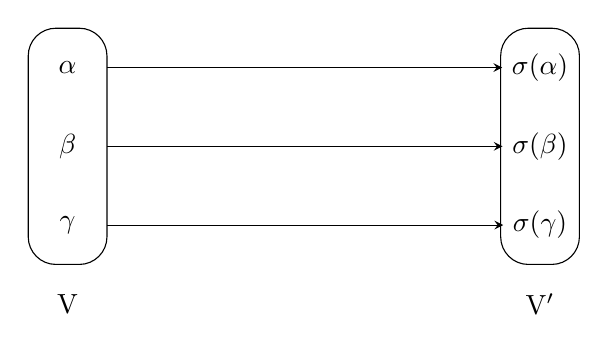
\begin{tikzpicture}[>=stealth]
        \draw[rounded corners=1em] (0, 0.5) rectangle (1, 3.5);
        \draw[rounded corners=1em] (6, 0.5) rectangle (7, 3.5);
        \node (A1) at (.5, 3) {$\alpha$};
        \node (B1) at (.5, 2) {$\beta$};
        \node (C1) at (.5, 1) {$\gamma$};
        \node (A2) at (6.5, 3) {$\sigma(\alpha)$};
        \node (B2) at (6.5, 2) {$\sigma(\beta)$};
        \node (C2) at (6.5, 1) {$\sigma(\gamma)$};
        \node at (.5, 0) {${\rm V}$};
        \node at (6.5, 0) {${\rm V'}$};
        \draw[->] (A1)++(.5, 0)--(A2);
        \draw[->] (B1)++(.5, 0)--(B2);
        \draw[->] (C1)++(.5, 0)--(C2);
    \end{tikzpicture}
    \caption{映射关系图}
    \label{映射关系图}
\end{figure}

% \begin{figure}[!htb]
%    如下图所示:
%         \ctikzfig{Chapter/TikZ/Visaul_Mapping}
%         \caption{映射关系图}
% \end{figure}

\noindent\num{1}\quad  $\alpha+\beta=\gamma \Rightarrow \sigma(\alpha)+\sigma(\beta)=\sigma(\gamma)$.
前面相等决定了后面一定相等\\
\num{2}\quad 因为是双射,所以我们也可以认为是$V'$中的每个元素都会被$V$中的元素所决\\ 
\num{3}\quad 我们把映射$\sigma$取逆,则可知:$V$中的每个元素被$V'$中的两个元素确定\\ 
\num{4}\quad 从2, 3点我们可以知道:$V$与$V'$中的对应元素的关系相同\\    

\begin{corollary}[线性空间的结构]
   所以我们可以认为线性空间的结构就是:\\ 
   \num{1} 元素的个数\\ 
   \num{2} 元素之间的关系(我们定义的加法和数乘)
   
   综上:

$\sigma(\sigma^{-1})$的存在,使得$V(V')$中的元素均被$V'(V)$中的元素确定。确定了数乘与加法以及相同的元素个数,所以$\sigma (\sigma^{-1})$使得$V$与$V'$有了不同的结构。           
\end{corollary}


\clearpage
\subsection{同构的线性空间具有相同的维数的证明}
\begin{proof}{\bf 错误的证明}\par
    如图\ref{映射关系图}所示:$\sigma: \alpha_i - \beta_i, ~\alpha_i \in V, \beta_i \in V'$
    是一个线性同构映射(只能够 $1-1$对应),那么我们就有
    \begin{align*}
        &\sigma(\alpha+\beta) = \sigma(\alpha) +\sigma(\beta)\\
        & \sigma(k\alpha) = k \sigma(\alpha)
    \end{align*}
    假如两个向量空间
    中的基向量的个数不相同,那么肯定不能够实现 $1-1$对应,所以矛盾。

    \bigskip
    ~~若 $V$的基为 \{\seq{\alpha}\}, $V$中的向量 \{\seq[s]{\beta}\} (不一定是基)。
    令 $\sigma(\alpha_i) = \sigma(\beta_i)$, 其中 $s>n$,则有
    \begin{align*}
        k_1\alpha_1 + \cdots + k_n\alpha_n = 0, \mathtext{其中} k_i = 0
    \end{align*}
    那么一定有
    \begin{align*}
     & \sigma(k_1\alpha_1 + \cdots + k_n\alpha_n)
        \rightarrow\mathtext{根据法则1:因为} k_i\alpha_i \in V\\ 
    =& \sigma(k_1\alpha_1) + \sigma(k_2\alpha_2 + \cdots + k_n\alpha_n)
        = \sigma(k_1\alpha_1) + \sigma(k_2\alpha_2) + \sigma(k_3\alpha_3 + \cdots + k_n\alpha_n)\\
    ~&\vdots\\
    =& \sigma(k_1\alpha_1) + \sigma(k_2\alpha_2) + \cdots + \sigma(k_n\alpha_n)
        \rightarrow \mathtext{根据法则2:} k_i\alpha_i \in V'\\
    =&  k_1\sigma(\alpha_1) + k_2\sigma(\alpha_2) + \cdots + k_n\sigma(\alpha_n)
        = k_1 \beta_1 + \cdots + k_n\beta_n\\
    =& 0
    \end{align*} 
    又因为 
    \[
    \displaystyle \sum_{i=1}^{n}{k_i\alpha_i}  = \sigma(\theta) = \theta
    = \sigma(\sum_{i=1}^{n}{k_i\alpha_i})
    = \sum_{j=1}^{n}{k_j\beta_j}
    = \theta\Rightarrow k_i = 0
    \]
    所以就可以得出 $\dim(\beta) \ge n$

    若 $\dim(\beta) \ge n$ 令 \seq[s]{\beta}, ~~(s>n),
    由于 $\sigma$ 是双射, 所以存在逆映射 $\sigma^{-1}$,
    使得
    \[
        \sigma^{-1}(\beta) = \alpha    
    \]
    同理,仿照上面的证明过程我们可以得到
    \[
        \dim(\alpha) \ge n
    \] 
    因为 $\beta_i, ~~i\in \{1, 2, \cdots, s\}$线性无关,则:
    \im{\sum_{i=1}^{s}{k_i\beta_i}}中 $k_i=0 \Rightarrow$ 
    \im{\sigma(\sum_{i=1}^{s}{k_i\beta_i})=\theta}, 
    即 
    \[
    \im{\sum_{i=1}^{s}{k_i\sigma(\beta_i)} = \sum_{i=1}^{s}{k_i\alpha_i} = \theta}
    \]
    那么就可以得到 $\dim(\alpha)>n$, 然而这与 $\dim(\alpha)=n$矛盾。
    于是可以得证:同构的线性空间具有相同的维数
\end{proof}

\begin{proof}{\bf 正确的证明}

    构造映射 $\sigma: \alpha_i - \beta_i, ~\alpha_i \in V, \beta_i \in V'$
    是一个线性同构映射(只能够 $1-1$对应),那么我们就有如下的两条性质:
    \begin{align*}
        &\sigma(\alpha+\beta) = \sigma(\alpha) +\sigma(\beta) \tag{1}\\
        & \sigma(k\alpha) = k \sigma(\alpha) \tag{2}
    \end{align*}

    \bigskip
    ~~若 向量空间$V$的基向量为 \{\seq{\alpha}\}, 向量空间$V'$中的向量 \{\seq[s]{\beta}\} (不一定是基)。
    构造一个向量。注:以下均假设 $\theta$是一个零元素(零向量):
    \[ 
    \im{\alpha = \sum_{i=1}^{n}{k_i\alpha_i} = \theta}
    \]
    因为 $\alpha_i$是 $V$的基。 所以$k_i=0$是上述方程的唯一解,于是有:

    \begin{minipage}[c]{0.3\linewidth}
        \vspace*{0pt}
        \begin{align*}
            \sigma(\sum_{i=1}^{s}{k_i\alpha_i})
            &\xlongequal[]{\mbox{\tiny 性质(1)}}  \sum_{i=1}^{s}{\sigma(k_i\alpha_i)}\\
            & \xlongequal[]{\mbox{\tiny 性质(2)}}  \sum_{i=1}^{s}{k_i\sigma(\alpha_i)}\\ 
            & =  \sum_{i=1}^{s}{k_i \beta_i} = \sum_{i=1}^{s}{\sigma(\alpha)} \\
            & =  \sum_{i=1}^{s}{\sigma(\theta)} = \theta\\
        \end{align*}
    \end{minipage}
        \hfill
    \begin{minipage}[c]{0.65\linewidth}
        \vspace*{0pt}
        \begin{formal}{blue!20}
            在这里说明,若 $\exists k_i \neq 0$, 则有矛盾;
            因为 $\sigma$是双射, 故存在唯一的逆映射 $\sigma^{-1}$,使得:\\
            \hspace*{3em}\im{\sigma^{-1}:~ \beta_i \rightarrow \alpha_i, ~ \beta_i \in V', \alpha_i \in V}  \\
            同样满足方程(1)(2),于是就有:\\
            \hspace*{1em}\im{
                \sigma^{-1} (\sum_{i=1}^{s}{k_i\beta_i}) 
                 = \sum_{i=1}^{s}{k_i\sigma^{-1}(\beta_i)}
                 = \sum_{i=1}^{s}{k_i\alpha_i} = \theta
            }\\
            若存在 $k_i\neq 0$, 那么就与前面的 $k_i=0$ 矛盾。 
        \end{formal}
    \end{minipage}

    \bigskip
    故 $\beta_i$ 线性无关。所以可以知道:$\dim(V')\ge n$, 下面证明若 $\dim(\beta)> n$则矛盾,若推出了矛盾,
    也就证明了 $\dim{V'} = n = \dim{V}$。不妨设 \seq[s]{\beta}为 $V'$的基,则
    \begin{align*}
        \sigma(\sum_{i=1}^{s}{l_i\beta_i}) = \sum_{i=1}^{s}{l_i\sigma(\beta_i)} = \sum_{i=1}^{s}{l_i\alpha_i}
    \end{align*}
    令 \im{\beta = \sum_{i=1}^{s}{l_i\beta_i} = \theta} , 则根据前面的证明过程可以知道 $l_i=0$,是此方程的唯一解。
    又因为解的唯一性,并且有 \im{\sigma(\theta) = \theta = \sum_{i=1}^{s}{l_i\alpha_i}},故 $l_i=0$是唯一解.
    所以可以得出 $V$的基向量个数为 $s(>n)$, 但是这与 $\dim(V)=n$ 矛盾。\textsf{证毕} $\square$
\end{proof}

\subsection{一个思考}
\begin{formal}{blue!20}
    \textsf{思考一:同解问题}\par 
    \ttfamily
    其实我认为这里有一个 $\sigma$映射下的同解性问题. 即:若方程
    \[
        \sum_{i=1}^{s}{k_i\alpha_i} = 0 \tag{*}
    \]
    有解 $\vec{K} = \{k_1, \cdots, k_s\}$
    我在上述方程的两边同时做映射 $\sigma$,那么可以得到 
    \[
        \sigma(\sum_{i=1}^{s}{k_i\alpha_i}) = \sigma(\theta) = \theta     \tag{**}
    \]

    于是可以知道方程 (**)的解为方程(*)的解。
    也就是说方程 (*)和方程 (**)同解, 即 $\sigma$ 作用下方程同解。
    因为 映射 $\sigma$ 只有
    作用于 零元素才可以得到零元素(向量空间的性质).
    \begin{center}
        若 $\sigma$是线性同构映射~$\Rightarrow \sigma(\alpha)= \beta$的$\alpha$是唯一的
    \end{center}
\end{formal} 


\begin{formal}{blue!20}
    \textbf{思考二:线性同构与线性变换的区别}\par 
    在线性变换中我们有:若 $\mathscr{A}$为一个线性变换,
    令 $k_1\alpha_1 + \cdots + k_n\alpha_n = \theta$,则我们可以得到:
    \[
        \mathscr{A}(k_1\alpha_1 + \cdots + k_n\alpha_n) = k_1\mathscr{A}(\alpha_1) + \cdots + k_n\mathscr{A}(\alpha_n) = \theta   
    \] 
    这里的变换 $\mathscr{A}$不是 $1-1$映射,其实就是使得 $\mathscr{A}(\gamma)=\theta$的 $\gamma$不是唯一的。

    结合上边的例子来解释就是:
    \[
        \mathscr{A}\im{\left(\sum_{i=1}^{s}{k_i\alpha_i}\right) = \theta \nRightarrow \sum_{i=1}^{s}{k_i\alpha_i}=\theta} 
    \]
    也就是说若 $\vec{K_0} = \{k_1, \cdots, k_s\}$是方程 \im{\sum_{i=1}^{s}{k_i\alpha_i}}的解,我们可以得到:
    \[
        \sum_{i=1}^{s}{k_i\alpha_i} = \mathscr{A}(\theta) = \theta
    \]
    但是如果我们有:
    \[
        \mathscr{A}\im{\left(\sum_{i=1}^{s}{k_i\alpha_i}\right)} = \theta
    \]
    那么此时 $K_0$肯定是这个方程的 \textbf{一个}解,但是这个方程很可能还有其他的非零元解
    (因为变换 $\mathscr{A}$不一定可逆, 它可以把一个非零向量 ${\sum\limits_{i=1}^{s}{k'_i\alpha_i}=\theta,~k'\neq k}$映射为一个零元素)。
    我们把这个解记为 $K'$, 那么明显 $K'\neq K_0$。也就是说此时满足:
    \im{
        \mathscr{A}\im{\left(\sum_{i=1}^{s}{k_i\alpha_i}\right)} = \theta
    }
    的解 $K'$, 不能够满足方程\im{\sum_{i=1}^{s}{k_i\alpha_i}=\theta}
\end{formal}

\clearpage